% Project Specifications

\chapter{Objects of Experiment}

\section{Keravan biomass power plant system}
\subsection{Overview of Keravan biomass power plant}
Keravan Energy is the main provider of electricity and district heating for the whole Kerava and Sipoo municipality in Southern Finland; they also sell electricity to many parts in Finland as well. Their electricity and district heating are solely produced at Keravan bio energy plant (Keravan bioboimalaitos).\cite{kerava:web}

The biomass power plant's production covers about 75 percent of Kerava city's district heating needs and about 25 percent of Keravan Energy's electricity purchase. The biomass power plant generates electrical power roughly at the rate of 21 megawatts (MW); process heat power generating capacity of about 10 MW and district heating power of about 50 MW. The power plant's boiler is fed by domestic fuels from clean wood (branches, barks, chips, twigs, stumps and etc) and milling cuttings. The principle process of the biomass power plant is illustrated in Figure \vref{fig:biomass}.

\begin{figure}[h]
  \centering
  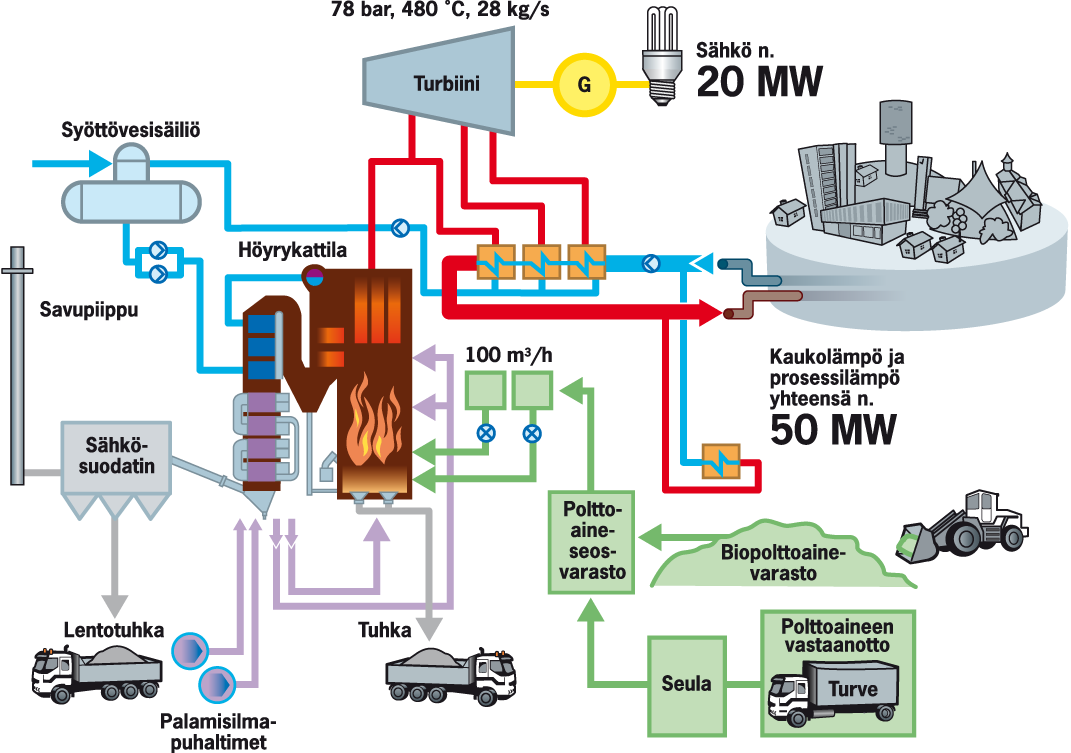
\includegraphics[width=7.5cm]{biomass}
  \caption{ Keravan Energy's biomass power plant working principles chart (Copied from keravanenergia.fi)(2018) \cite{kerava:web}).}
  \label{fig:biomass}
\end{figure}

The power plant was built following the principles of Best Available Techniques (BAT). The wood and biomass fuel is received and screened before going into a fuel mixture storage. These mixed wood fuels are fed into a kerosene boiler. In combustion chamber, the fuels are burned and released combustion gases. These gases go through and heated feed water from feeding water tank. Theses gases goes through another cooling system to get into electrostatic precipitator to precipitate fly ash. The exhausted gases from the chimney are already dedusted, damped and desulphurised and safe for environment. The bottom ash of boiler is reused in chamber and collected afterward. In the pipe from the boiler there is high pressure steam going to drive a turbine. The generator converts kinetic energy from turbine to electricity for municipality. The heat is used for district heating networks. Then the remaining steam is condensed in a condenser which acted as circulating  feeding water for boiler again.
\subsection{Piping cooling section}
The targeted piping section in our experiment is a part of equipment for ash handling system in Keravan biomass power plant. The cooling system helps reducing the heat of flying ash in order to help them land down on the surface for ash collection. Figure \vref{fig:original_pipe} shows a original piping section that we are going to use for the test. 

\begin{figure}[h]
  \centering
  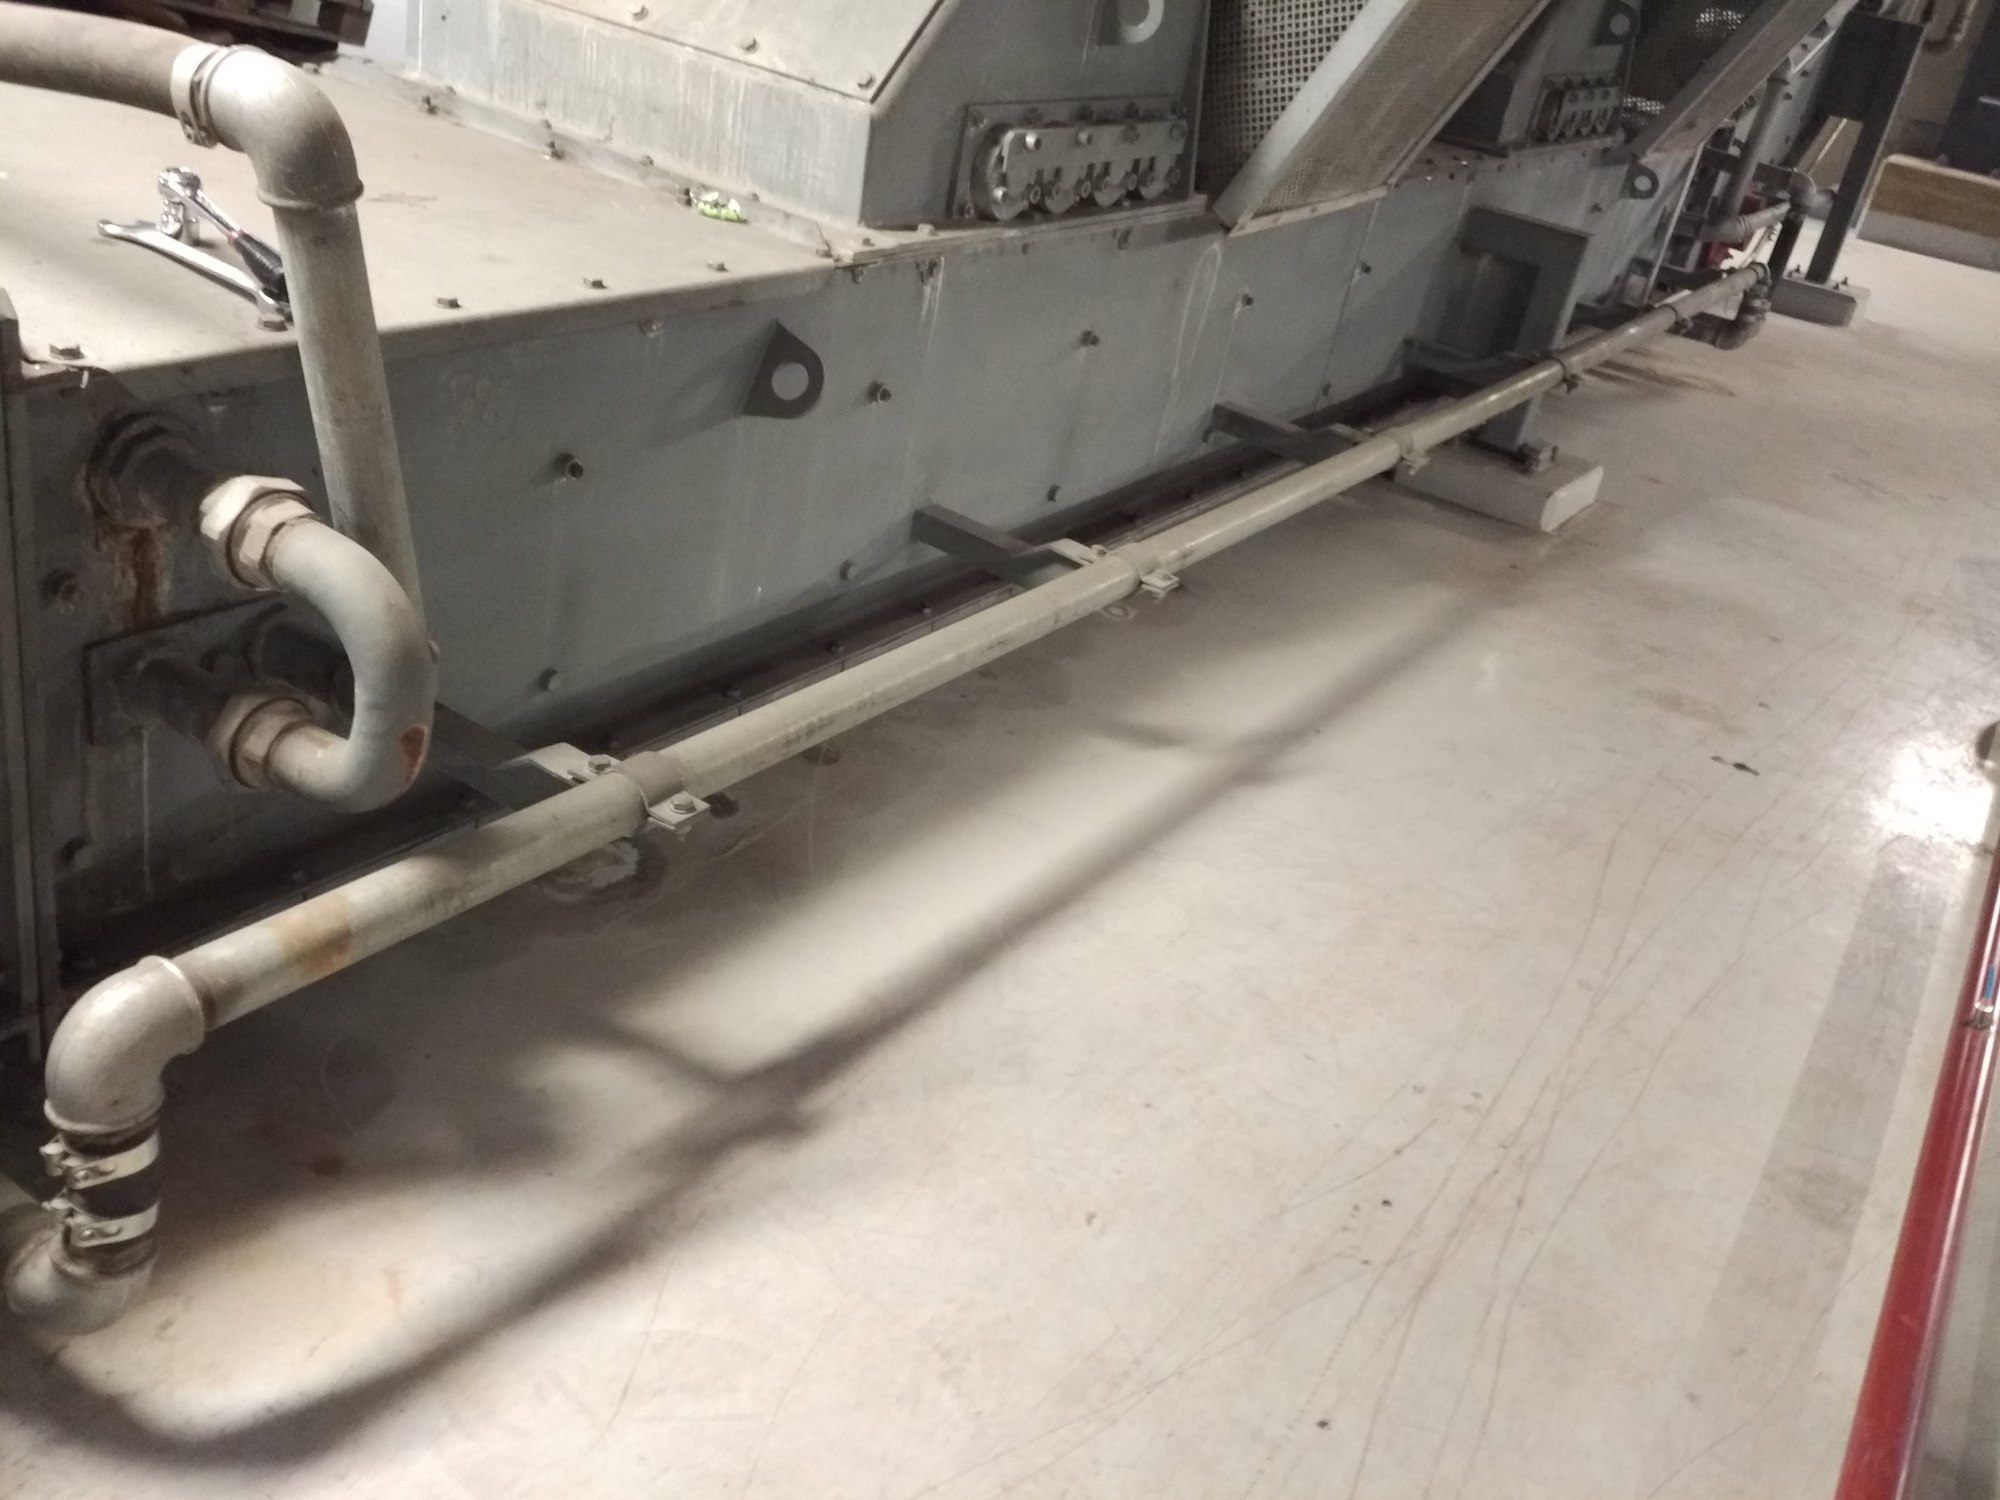
\includegraphics[width=7.5cm]{original_pipe}
  \caption{ Targeted piping section altered in the experiment}
  \label{fig:original_pipe}
\end{figure}


\section{Voxer}
\subsection{Static Mixer}

\subsection{Principle Design}
As it is mentioned above, the half elliptical shape of Voxer is inspired by semi-elliptical structure of many kinds of motionless mechanical mixer.Voxer, which includes a vortex flow wing and a tube, was designed by Chief Engineer of SansOx Ltd., Juhani Pylkkänen. Voxer's design is relatively simple. It is made of thin stainless steel plate with flat profile, which can be put into functional form by twisting and stretching (see Figure \vref{fig:voxer2}). The surfaces of Voxer are simply refined; the edges are rounded. It can be customized and installed easily inside any kind of circular tube (see Figure \vref{fig:voxerpipe}). The water flow in pipe would twist the Voxer tightly to the inner surface of the pipe which has no cross beam. Figure \vref{fig:voxer1} illustrates the design that mitigates the stresses and losses on its own structure; so it can be installed with a tight fit that prevents it from rotating \cite{voxer:article}.

\begin{figure}[h]
  \centering
  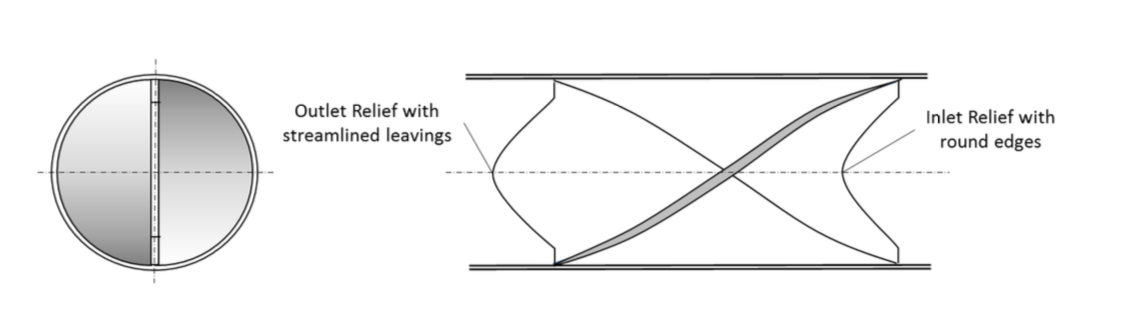
\includegraphics[width=7.5cm]{Voxer_view1}
  \caption{ Fixation of Voxer in pipe \cite{voxer:article}}
  \label{fig:voxer1}
\end{figure}

\begin{figure}[h]
  \centering
  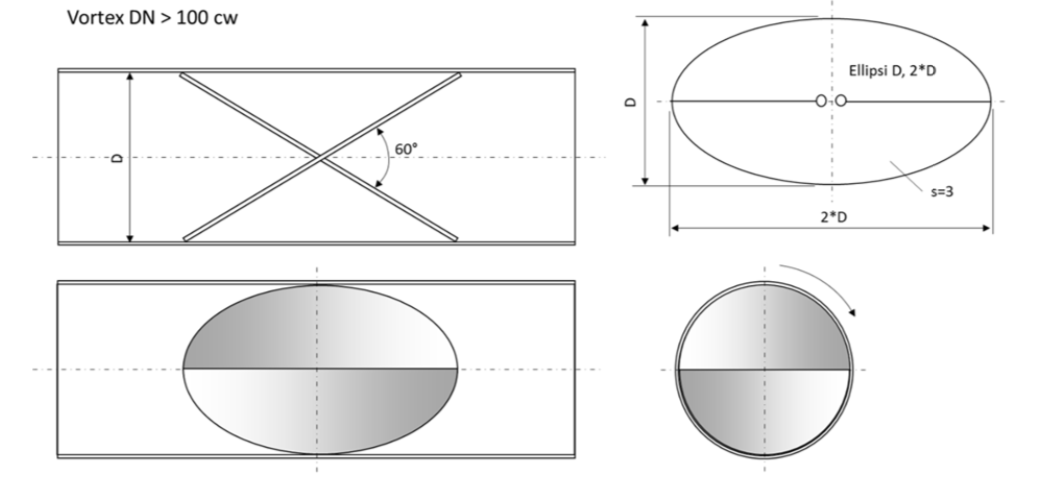
\includegraphics[width=7.5cm]{Voxer_view2}
  \caption{ View of Voxer's design \cite{voxer:article}}
  \label{fig:voxer2}
\end{figure}

\begin{figure}[h]
  \centering
  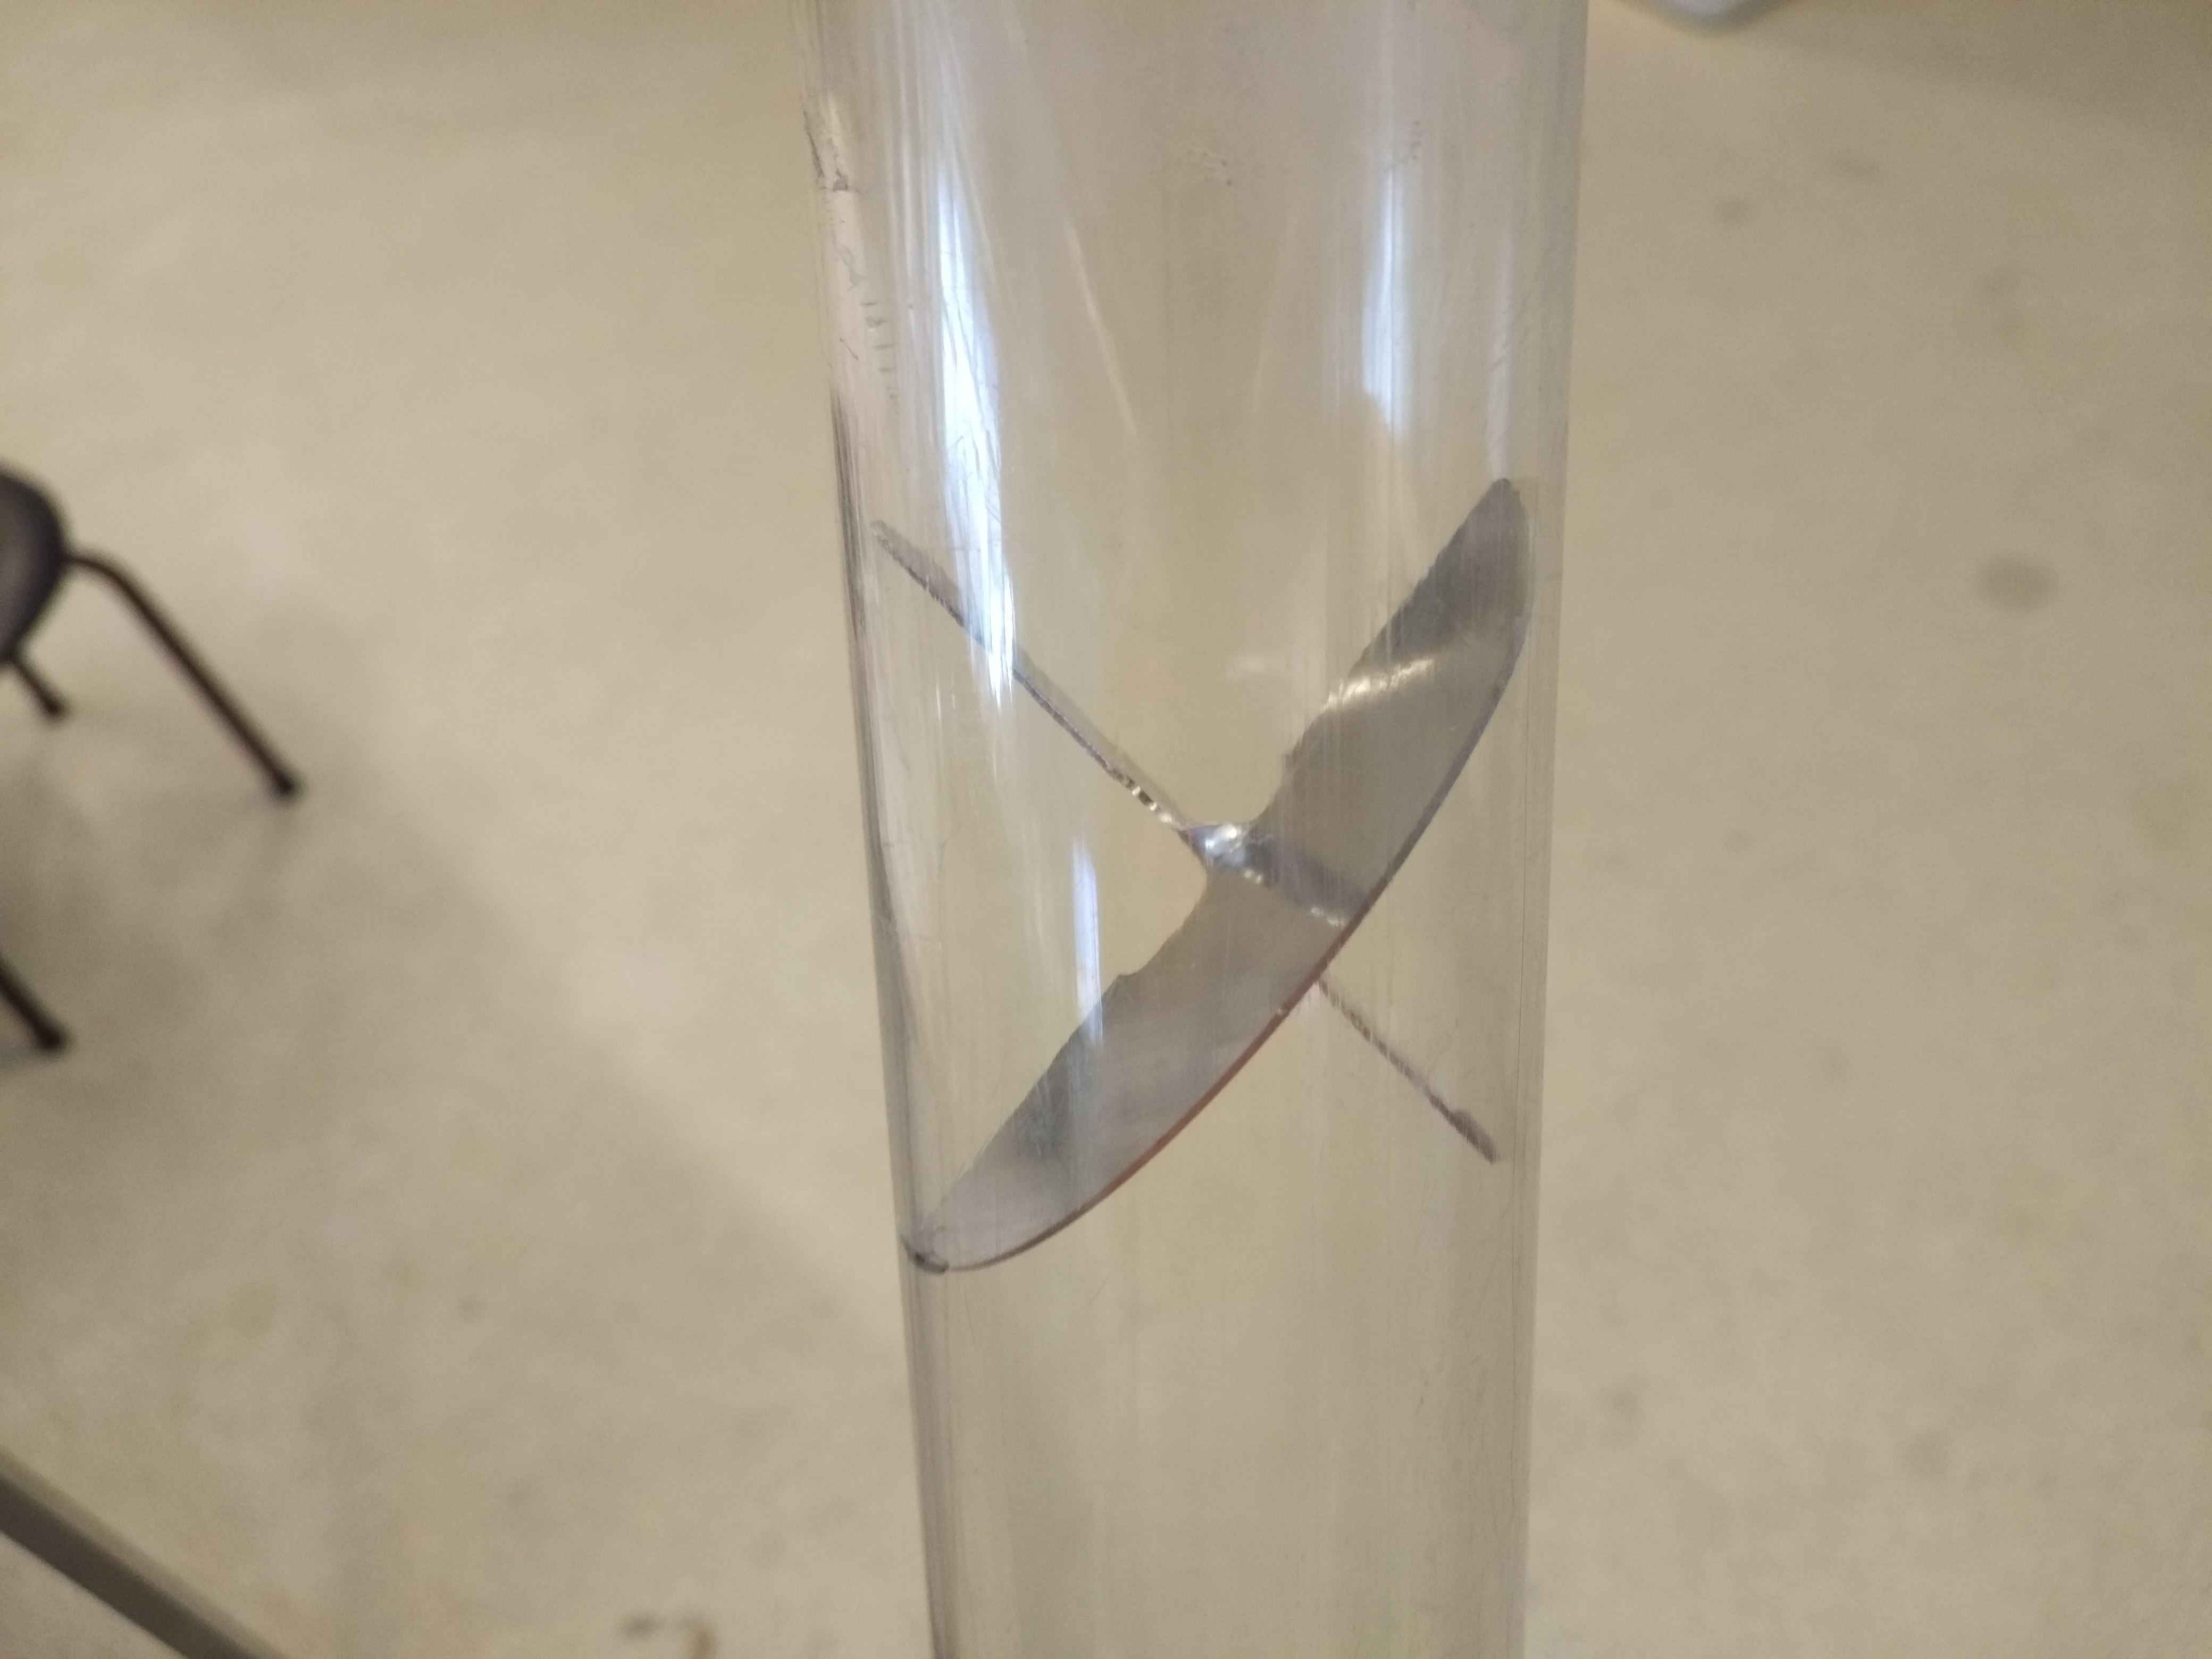
\includegraphics[width=7.5cm]{voxer_inpipe}
  \caption{ Elliptical Voxer wing in transparent pipe}
  \label{fig:voxerpipe}
\end{figure}
\subsection{Functions}
Mr. Pylkkänen described that the vortex wing of Voxer is going to decrease turbulences and flow losses in a tube, where liquid or gas flows by gravity or pressure \cite{voxer:article}. The vortex wing generates vortex flow which smoothen the rotation of mass flow around the tube centerline. Figure \vref{fig:flow} and figure \vref{fig:flowprofile} illustrate how the blade divides the original flow into two equal vortex flows. The flow speed profile is getting flatter while the flow speed close to tube inner surface increases. It reduces the boundary of no-slip condition of the flow near inner pipe surface. We can see in figure \vref{fig:flowprofile} the impact of Voxer wing on forming the vortex flow is more and more significant in curves. In the curves up to 90 degree, losses with Voxer are similar to the straight tube with the same diameter. 
\begin{figure}[h]
  \centering
  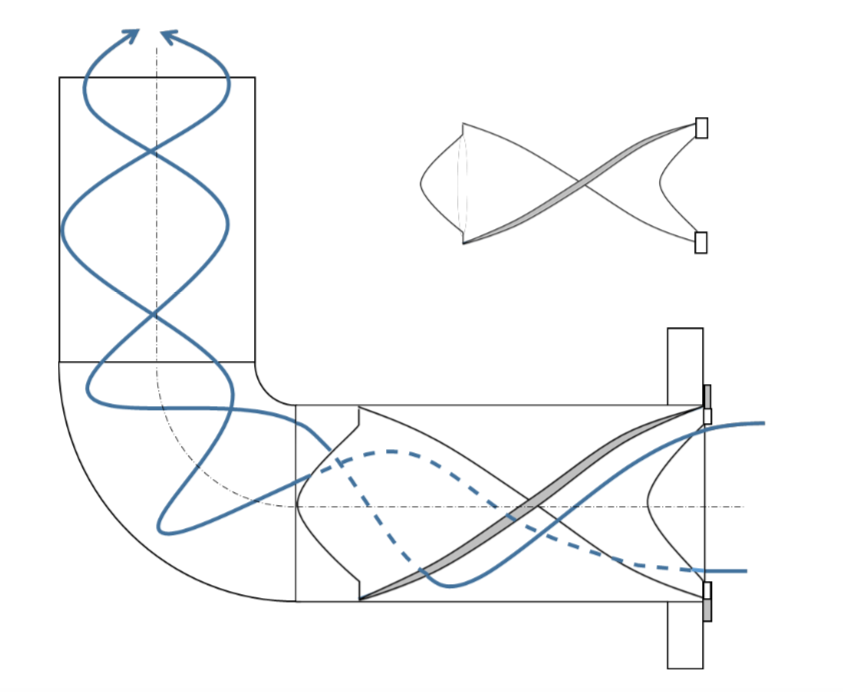
\includegraphics[width=7.5cm]{flowinpipe}
  \caption{ Flow graph in a 90 degree curve\cite{voxer:article}}
  \label{fig:flow}
\end{figure}
\subsection{Economical value}
\begin{figure}[h]
  \centering
  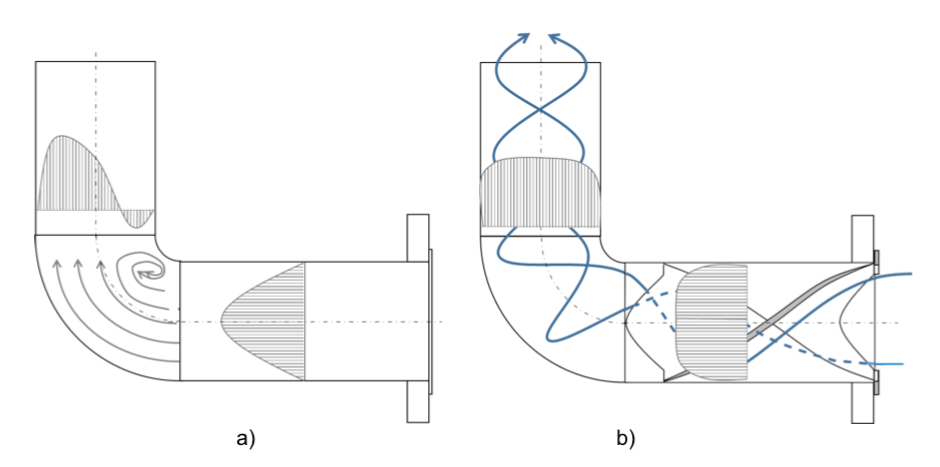
\includegraphics[width=7.5cm]{flow_profile}
  \caption{ Flow speed profile in straight tube and curve \newline a) without Voxer and b) with Voxer. \cite{voxer:article}}
  \label{fig:flowprofile}
\end{figure}

In the following figures, we can compare the differences between water flow without and with Voxer wing at the same flow velocity. Turbulences occur in and after the curves in figure \vref{fig:vox1}, which indicates flow losses and energy losses in the flow. The behavior of flow in figure \vref{fig:vox2} is comparable with the flow profile figure \vref{fig:flowprofile}. The flow is smoothened with reduced pressure in vortex center and no turbulence occurs.
\begin{figure}[h]
  \centering
  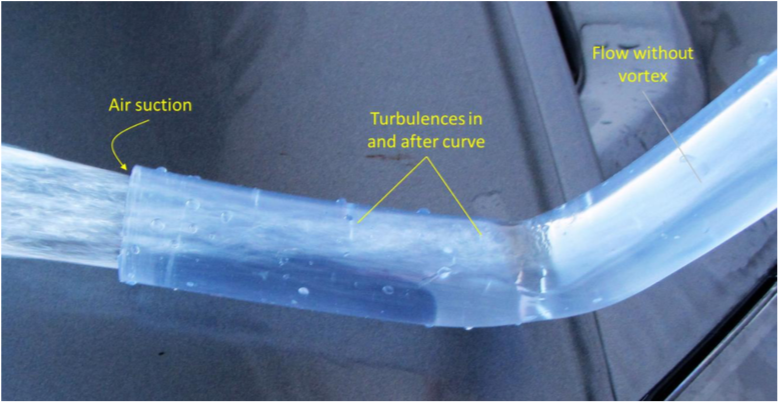
\includegraphics[width=9cm]{no_voxer}
  \caption{ Regular water without vortex effect.\cite{voxer:article}}
  \label{fig:vox1}
\end{figure}
\begin{figure}[h]
  \centering
  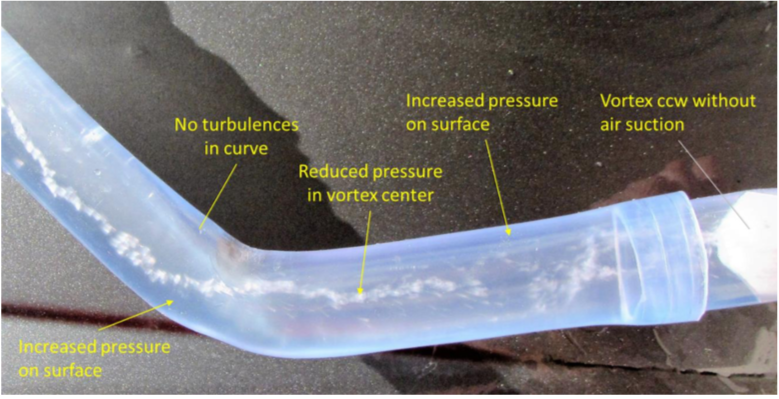
\includegraphics[width=8cm]{with_voxer}
  \caption{ Vortex water flow with same flow velocity.\cite{voxer:article}}
  \label{fig:vox2}
\end{figure}

\subsection{Economical value}
While the static mixer is more expensive and hard to request customized model for existing pipelines, Voxer is designed in accordance with economical and performance parameters. Apart from simple design, Voxer can be manufactured with reasonably cost-effective expense. In addition to cheaper product cost, Voxer is able to deliver many good benefits to customers with lower maintenance and operation cost.
With normal screw type of blade, it is needed to be scheduled to be produce during planning stage of pipeline system. Voxer with half cut elliptical blades can be fitted in any existing tube with big diameter. The flow is smoothly divided in to two equal vortex flows flowing in relation like rolling patterns on their contacts. Without the rolling effect, dirt is formed on cross beam of screw type blades at intake. Apparently the half ellipse installed the inner tube surface has no cross beam. Hence the blades stay clean and less maintenance is required. This is the best marketable technical feature of the Voxer. Moreover, Voxer has versatile compatibility with various liquids like water, wastewater, slurry, oil and different gases like air, oxygen, nitrogen, natural gas, carbon dioxide and hydrogen \cite{voxer:article}. 
\clearpage %force the next chapter to start on a new page. Keep that as the last line of your chapter!
